\section{"3" Оптимизация кинематической схемы}

\begin{frame}[t]{Определение количества ног}
    \framesubtitle{}
    \begin{columns}[T,onlytextwidth]
        \begin{column}{0.59\textwidth}
            \small
            Решить $F=f(x) \rightarrow max$, где

            $f(x)$ --- \textbf{ Критерии}: пройденная дистанция, длина корпуса\\
            $x$ --- \textbf{Параметры}: количество ног, сдвиг фазы между соседними ногами

            \textbf{Метод решения}: Генетический алгоритм: Open AI-ES

            \textbf{Алгоритм}: \underline{генерируется множество особей}, а
            также \underline{семейство территорий} с одинаковой сложностью.
            За фиксированное время, с постоянной угловой скоростью
            на моторах, каждый \underline{робот проходит это семейство
            территорий} и записываются данные.

            \textbf{Предположения}: 1) есть только \underline{сухое трение}
            между ногами и поверхностью. 2) Созданные
            поверхности с помощью \underline{одной функции
            и параметров} имеют \underline{одинаковую сложность}.

            \textbf{Утверждение}: \textit{Количество ног имеет прямую
                зависимость с длиной корпуса робота.}
        \end{column}
        \begin{column}{0.39\textwidth}
            \begin{figure}[H]
                \begin{subfigure}{0.49\textwidth}
                    \centering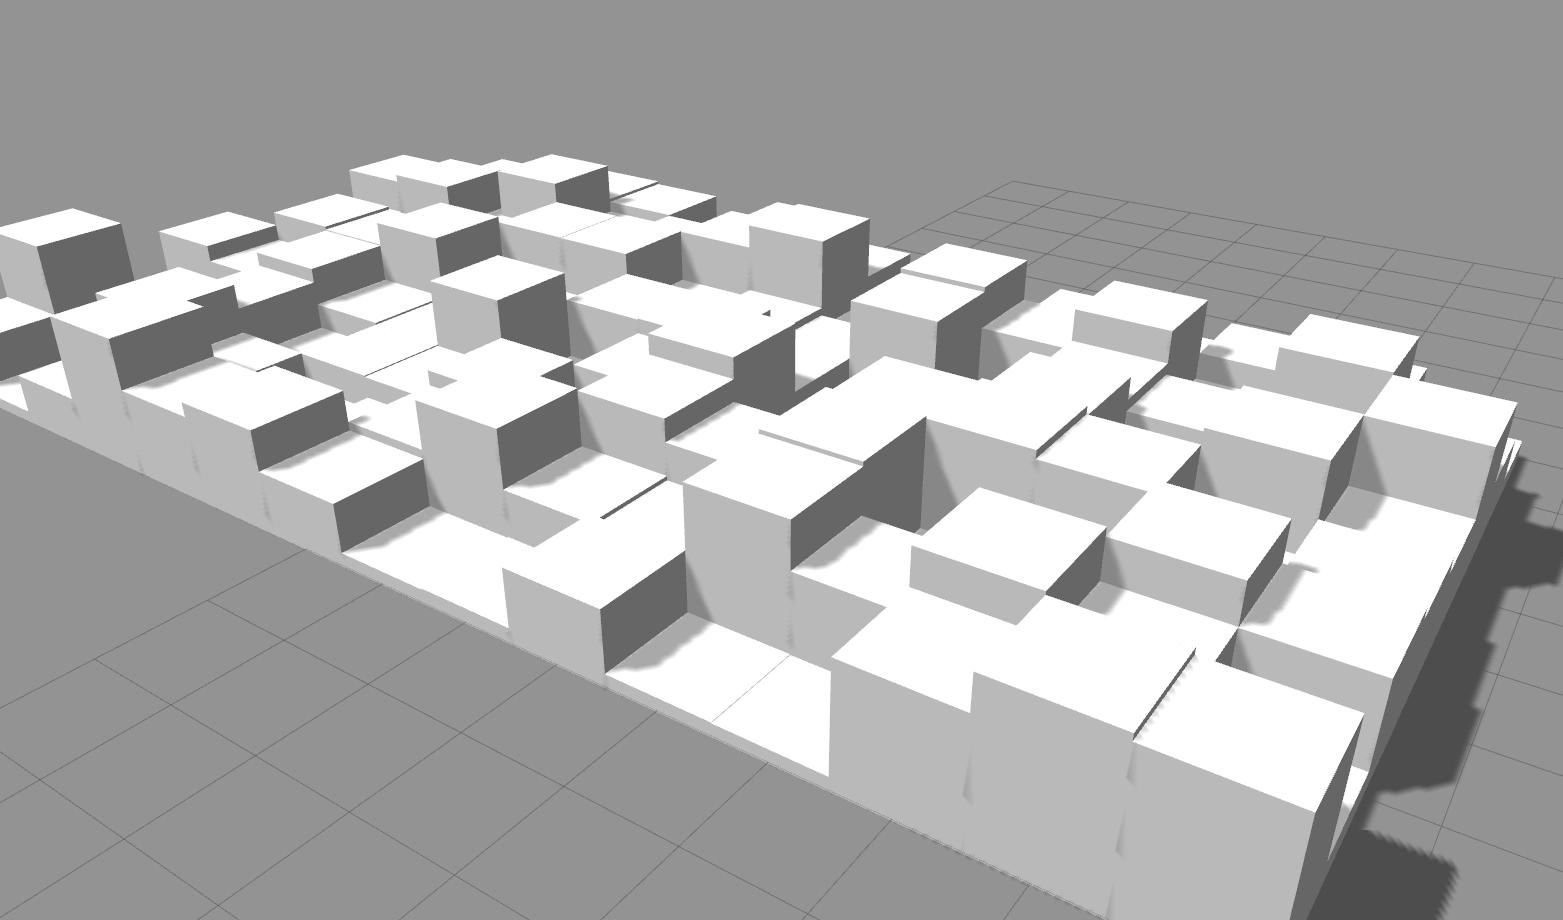
\includegraphics[height=2cm,width=1\textwidth,keepaspectratio]{../images/terrain_1.jpg}
                    \caption*{Равномерное распределение ячеек}
                \end{subfigure}
                \begin{subfigure}{0.49\textwidth}
                    \centering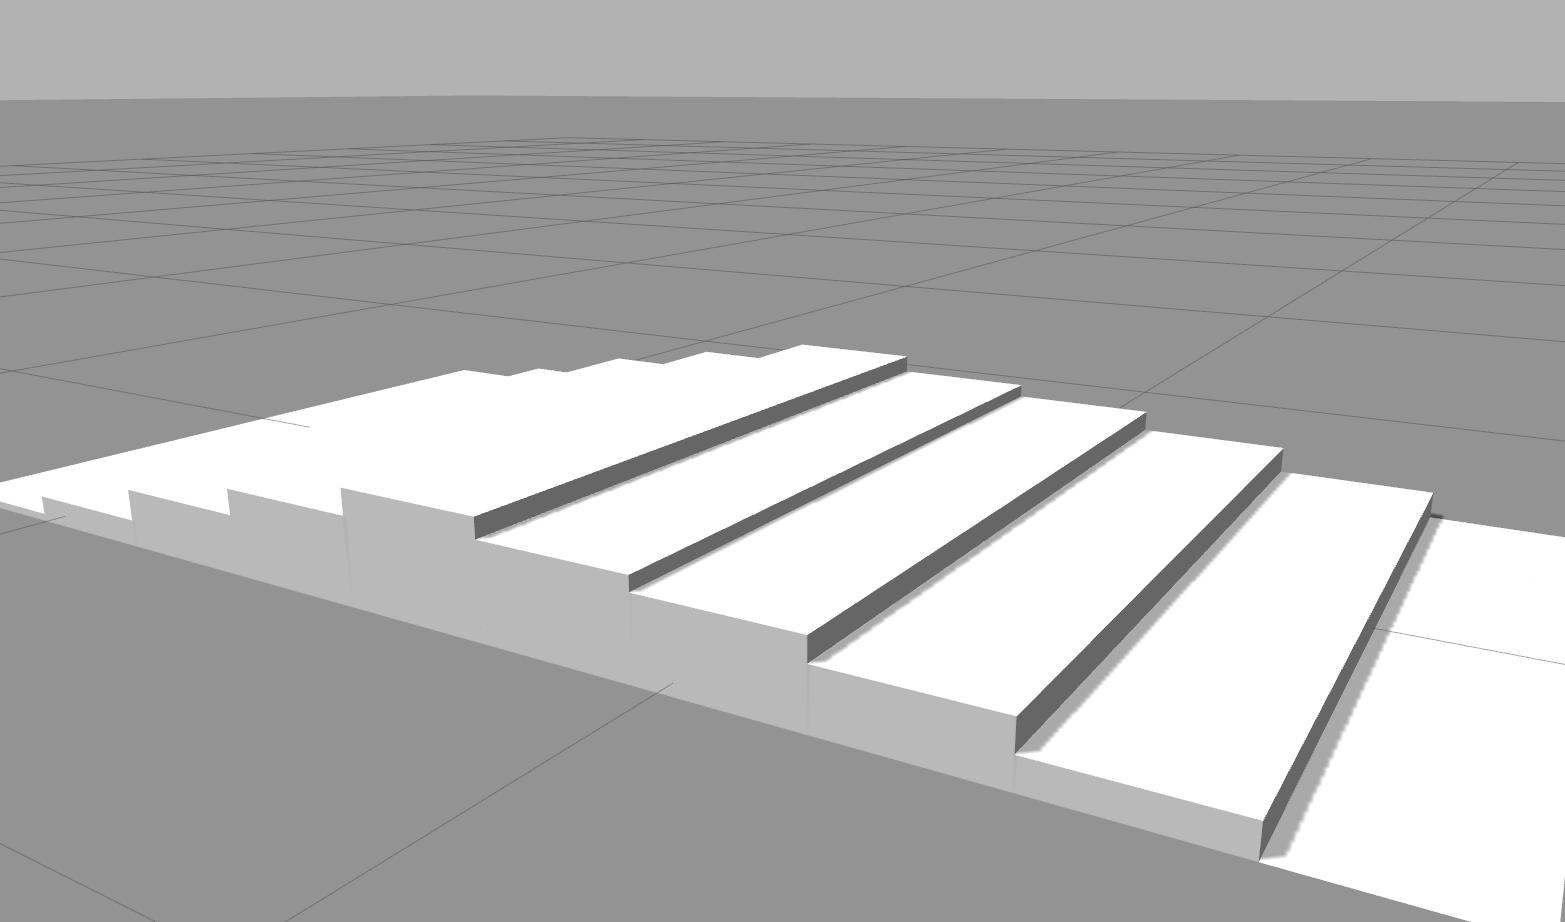
\includegraphics[height=2cm,width=1\textwidth,keepaspectratio]{../images/terrain_2.jpg}
                    \caption*{Гауссово распределение ячеек}
                \end{subfigure}

                \begin{subfigure}{0.99\textwidth}
                    \centering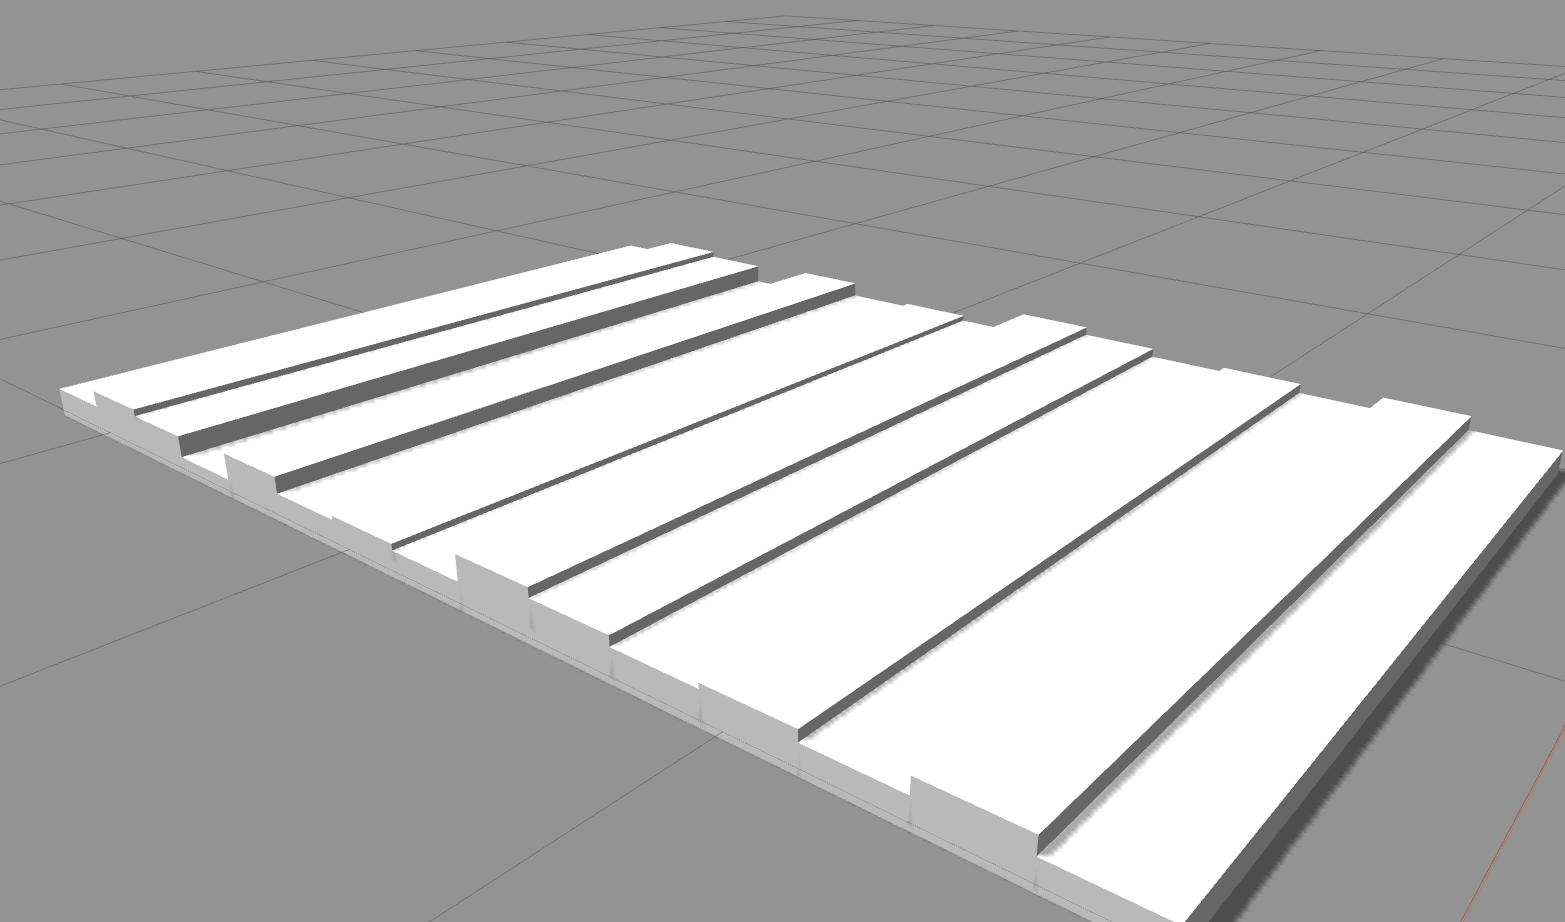
\includegraphics[height=2.8cm,width=1\textwidth,keepaspectratio]{../images/terrain_3.jpg}
                    % \caption*{Пример прохождения особью сгенерированной поверхности}
                \end{subfigure}
            \end{figure}
        \end{column}
    \end{columns}
\end{frame}

\note{\small \setlength{\parindent}{20pt}

Так как детализация покрытия опорной поверхности зависит от количества ног, то я решил начать с разработки робота. Первым его этапом было определение количества ног.

Было решено оценивать проходимость с помощью экспериментов, где робот с конкретным количеством ног проходит по семейству территорий с одинаковой сложностью за фиксированное время. На моторы подается постоянная угловая скорость. 

Семейства территорий с одинаковой сложностью - семейства, которые были сгенерированы с помощью одинаковых параметров. *тык* К примеру с помощью нормального распределения, где одинаковый параметр дисперсии.

Также было сделано предположение, что количество ног не сильно влияет на проходимость на гибридных поверхностях, такие как мох, поэтому рассматривается только сухое трение между ногами и поверхностью.

Задача решалась с использованием генетического алгоритма Open AI-ES.}



\begin{frame}[t]{Описание механической системы}
    \framesubtitle{}
    \begin{align}
        \boxed{M \dot{\vec{u}} = \vec{g}}                                \\
        M = \begin{bmatrix}
                M_1    & \cdots & 0      \\
                \vdots & \ddots & \vdots \\
                0      & \cdots & M_n
            \end{bmatrix},\ M_i = \begin{bmatrix}
                                      m_i E_{3\times 3} & 0   \\
                                      0                 & I_i
                                  \end{bmatrix}        \\
        \vec{u}_i^{\ T} = \begin{bmatrix}
                              \vec{v}_i^{\ T} & \vec{\omega}_i^{\ T}
                          \end{bmatrix} \\
        \vec{g}^{\ T} = \begin{bmatrix}
                            \cdots \  \vec{F}_i^{\ T}, & (\vec{\tau}_i - \vec{\omega}_i \times I_i \vec{\omega}_i)^T\  \cdots
                        \end{bmatrix}
    \end{align}
    где, $M_i$~---~матрица массово-инерционных характеристик; $m_i$~---~масса тела; $I_i$~---~тензор инерции; $\vec{u_i}$~---~вектор обобщённых скоростей; $E$~---~единичная матрица; $\vec{g}$~---~вектор обобщённых сил; $\vec{v_i}$~---~вектор линейной скорости; $\vec{\omega_i}$~---~вектор угловой скорости; $\vec{F_i}$, $\vec{\tau_i}$~---~силы и моменты сил взаимодействия.
\end{frame}

\note{\small \setlength{\parindent}{20pt}

Для симуляции работы робота необходимо описать его математическую модель. Рассматривалась механическая система из абсолютно твердых тел, состоящая из корпуса робота и некоторого количества ног. Так как количество ног меняется, то показаны обобщенные формулы.

Я расписал дифференциальные уравнения механической системы в известной форме *тык*. В английской литературе данный метод называется методом Ньютон Эйлера. 
}

\begin{frame}[t]{Наложенные связи}
    \framesubtitle{}
    Тела соединены цилиндрическими шарнирами:
    \begin{align}
        \phi(q_{j_1},\ \cdots,\ q_{j_k},\ t) \geqslant  0 \\
        \vec{q_i}^{\ T} = \begin{bmatrix}
                              \vec{x}_i^{\ T} & \vec{Q}_i^{\ T}
                          \end{bmatrix}                   \\
        \dot{\vec{q_i}} = \begin{bmatrix}
                              E_{3\times3} & 0            \\
                              0            & G(\vec{q}_i)
                          \end{bmatrix}\vec{u}_i
    \end{align}
    \begin{align}
        \vec{g}_i = \tau_i^T \vec{z}_{i-1} -k_i \dot{\vec{q_i}}
    \end{align}
    где $\phi$ --- функция связи; $t$~---~время; $\vec{q}_{i}$~---~вектор обобщенных координат, включающий в себя координаты центра масс $\vec{x_i}$ и кватернион $\vec{Q_i}$, описывающий ориентацию тела в пространстве; $G(\vec{q}_i)$ --- матрица, вид которой зависит от выбранной системы координат; $k$~---~ коэффициент вязкого трения в шарнире.
\end{frame}

\note{\small \setlength{\parindent}{20pt}

Эти дифференциальные уравнения дополнены связями. Тела соединены цилиндрическими шарнирами. Ориентация описана кватернионами, так как робот может переворачиваться и может возникнуть складывание рамок, если будем использовать углы Эйлера.

Хочется отметить, что в шарнире учитывается коэффициент вязкого трения.}

\begin{frame}[t]{Взаимодействие опорной поверхности и ноги робота}
    \framesubtitle{}
    \begin{columns}[T,onlytextwidth]
        \begin{column}{0.64\textwidth}
            \begin{align}
                \phi_u(\vec{q}\ ) \geqslant 0                                                     \\
                \phi_u(\vec{q}\ ) = (\vec{x}_1 + \vec{s}_1 - \vec{x}_2 - \vec{s}_2) \cdot \vec{n} \\
                \frac{d }{d t}\phi_u(\vec{q}\ ) \approx \begin{bmatrix}
                                                            \vec{n}^{\ T} & (\vec{s}_1 \times \vec{n})^T & -\vec{n}^{\ T} & (-\vec{s}_2 \times \vec{n})^T
                                                        \end{bmatrix} \begin{bmatrix}
                                                                          \vec{v}_1      \\
                                                                          \vec{\omega}_1 \\
                                                                          \vec{v}_2      \\
                                                                          \vec{\omega}_2 \\
                                                                      \end{bmatrix}
            \end{align}
            где, $\phi_u(\vec{q})$~---~функция связи; $ \mu $~---~ коэффициент трения между ногой и опорной поверхностью;  радиус-векторы $\vec{x}_{1,2},\ \vec{s}_{1,2}$ и орты координатных осей $\vec{t}_{1,2}, \vec{n}$ показаны на рисунке; $ f_{1,2} $~---~значения сил трения вдоль осей $t_{1,2}$.
        \end{column}
        \begin{column}{0.35\textwidth}
            \vspace{-0.4cm}
            \begin{figure}[H]
                \centering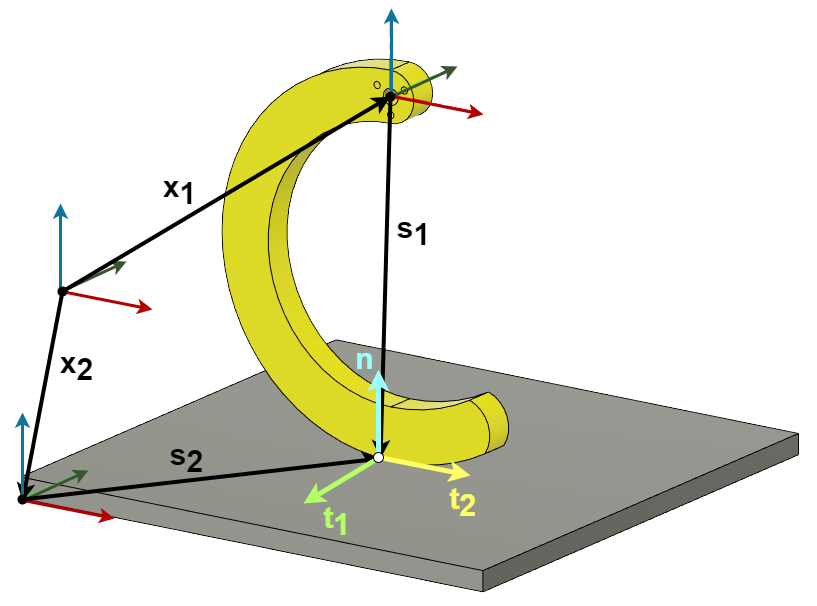
\includegraphics[height=6cm,width=1\textwidth,keepaspectratio]{contact_interaction.png}
            \end{figure}
            \vspace{-1cm}
            \begin{align}
                \left\{\begin{matrix*}[l]
                           \mu f_n \geqslant \sqrt{f_1^2 + f_2^2}\\
                           \left\lVert \vec{v_t}\right\rVert (\mu f_n - \sqrt{f_1^2 + f_2^2}) = 0\\
                           \dfrac{\vec{f_t}}{\left\lVert \vec{f_t}\right\rVert } = - \dfrac{\vec{v_t}}{\left\lVert \vec{v_t}\right\rVert }
                       \end{matrix*}\right.
            \end{align}
        \end{column}
    \end{columns}
\end{frame}

\note{\small \setlength{\parindent}{20pt}
Для шагающих роботов критично важно правильно описать взаимодействие с опорной поверхностью. Используется модель сухого трения, описанная конусом трения.

На рисунке *тык* предоставлено обозначение радиус векторов, для решения задачи направления сил реакции опоры и трения в общем виде.
}

\begin{frame}[t]{Целевая функция}
    \framesubtitle{}
    \begin{eqnarray}
        F \rightarrow max = \beta \left( {\omega}_{1} \cdot \delta + {\omega}_{2} \cdot L\right) + (1 - \beta) {\delta}^{{\omega}_{1}} {\left( L\right)}^{{\omega}_{2}} \\
        L = \frac{1}{(\gamma - 1) h_{\text{leg}}sin(\alpha)}
    \end{eqnarray}
    \begin{columns}[T,onlytextwidth]
        \begin{column}{0.48\textwidth}
            Где
            $\beta$ -- адаптивный параметр, \\ ${\omega}_{1,2} \in  [ 0..1 ] $ -- весовые коэффициенты, \\
            $\delta$ -- пройденный путь, \\
            $L$ -- упрощенная длина робота

            % \textit{Для решения однокритериальной задачи} использовалась аддитивно-мультипликативная свертка
        \end{column}
        \begin{column}{0.50\textwidth}
            \begin{figure}[H]
                \centering
                \centering\includegraphics[height=3cm,width=1\textwidth,keepaspectratio,page=3]{./tikz_pictures.pdf}
                \caption*{Геометрическое представление особи}
            \end{figure}
        \end{column}
    \end{columns}
\end{frame}

\note{\small \setlength{\parindent}{20pt}

Целевая функция выглядит следующим образом. В формуле дельта это пройденный путь, а L --- упрощенная длина робота, без лишних констант. Омеги --- весовые коэффициенты, их можно воспринимать следующим образом. Сумма коэффициентов равна 1. Настраивая данные коэффициенты можно показать, что в конкретной оптимизации важнее: проходимость или размеры робота. 

В данном прототипе подразумевалось, что ноги двигаются зависимо друг от друга, поэтому сдвиг фазы между соседними ногами влияет на длину робота. На рисунке объяснены компоненты формулы *тык*
}

\begin{frame}[t]{Закономерность}
    \begin{columns}[T,onlytextwidth]
        \begin{column}{0.49\textwidth}
            Лучшие роботы в экспериментах начинались с 10 до 14 ног для различных значений $\omega$.

            Это объясняется критерием статического равновесия. В таком случае минимум 4 ноги всегда касаются поверхности.
        \end{column}
        \begin{column}{0.49\textwidth}
            \begin{figure}[H]
                \centering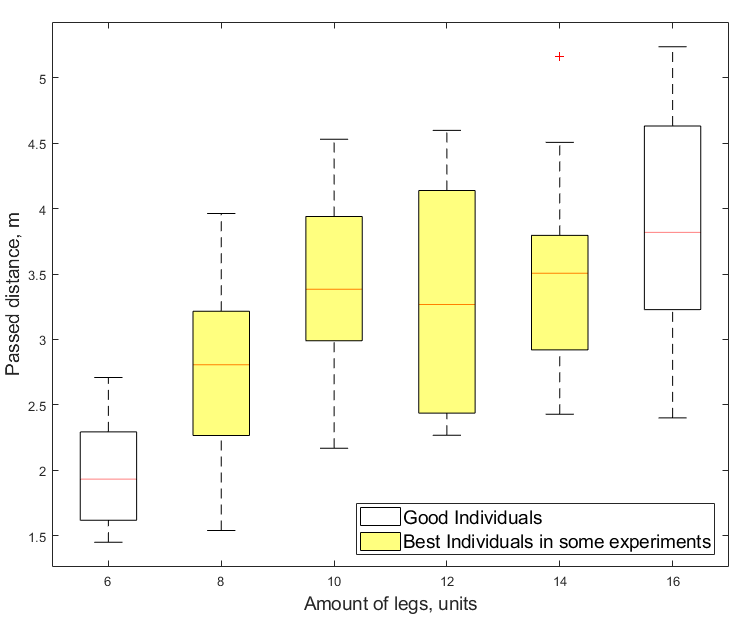
\includegraphics[height=5cm,width=1\textwidth,keepaspectratio]{box_plot_structural_synthesis.png}
                \caption*{Зависимость между кол-вом ног и пройденной дистанцией}
            \end{figure}
        \end{column}
    \end{columns}
\end{frame}

\note{\small \setlength{\parindent}{20pt}

Результатом оптимизации получена зависимость количества ног робота в зависимости от различных весов. пары омега тоже менялись. Этот массив данных собирался и был представлен в виде блочной диаграммы с ограничителями выбросов, где *тык* показаны квартили каждой выборки.

Лучшие результаты были получены, когда ног было от 10, до 14и.}

\begin{frame}[c]{Прототипы робота}
    \begin{figure}[H]
        \begin{subfigure}{0.32\textwidth}
            \centering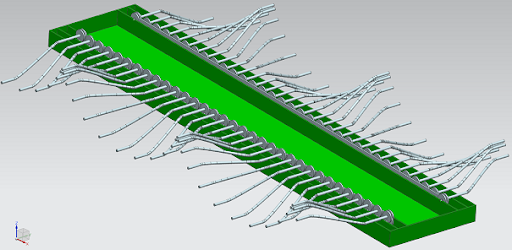
\includegraphics[height=3cm,width=1\textwidth,keepaspectratio]{strirus_0.png}
        \end{subfigure}
        \begin{subfigure}{0.32\textwidth}
            \centering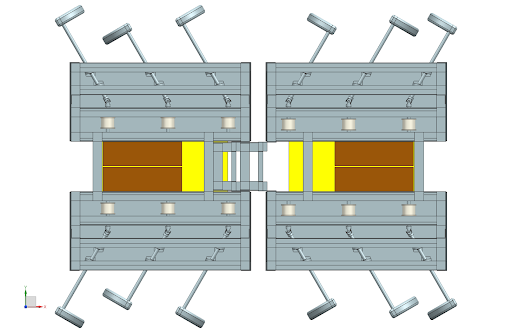
\includegraphics[height=3cm,width=1\textwidth,keepaspectratio]{strirus_1.png}
        \end{subfigure}
        \begin{subfigure}{0.32\textwidth}
            \centering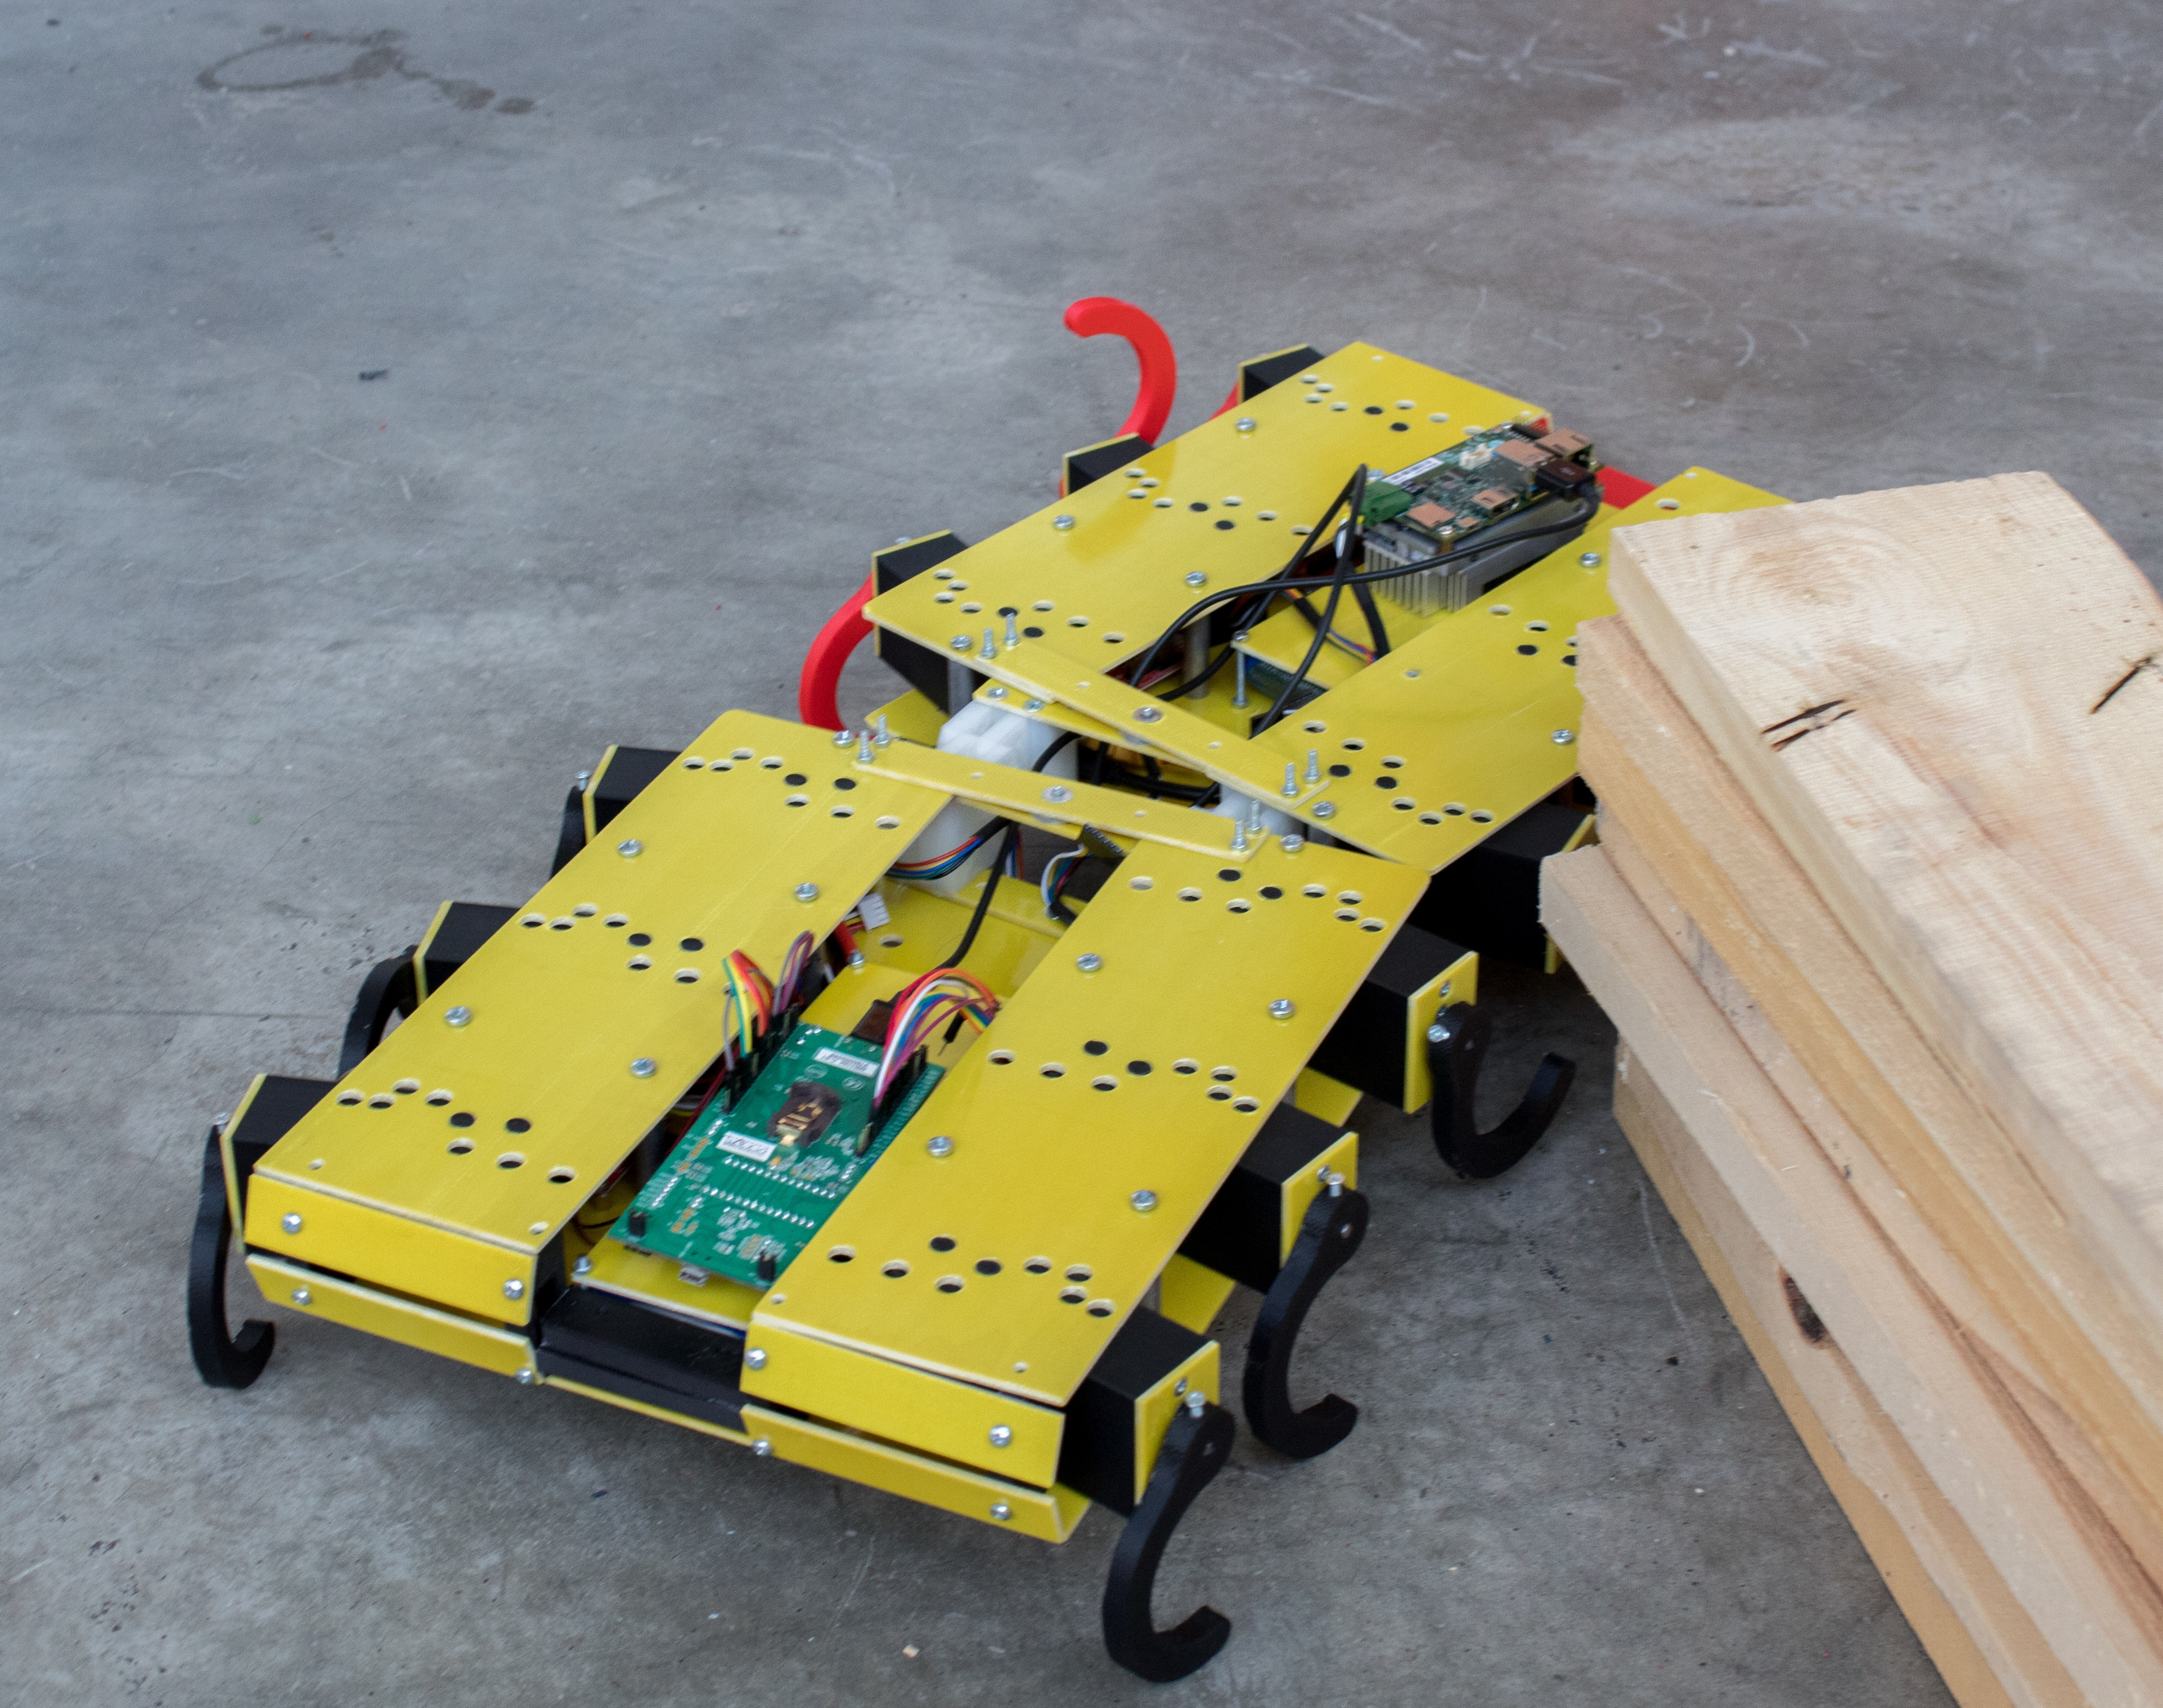
\includegraphics[height=3cm,width=1\textwidth,keepaspectratio]{strirus_2.jpg}
        \end{subfigure}

        \begin{subfigure}{0.32\textwidth}
            \centering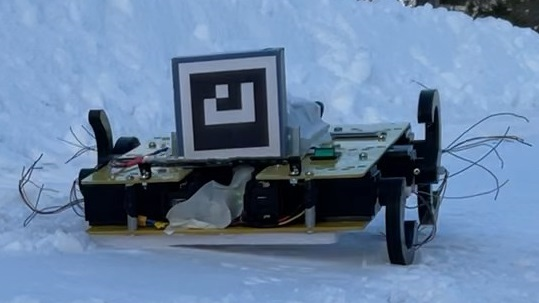
\includegraphics[height=3cm,width=1\textwidth,keepaspectratio]{strirus_3_snow.jpg}
        \end{subfigure}
        \begin{subfigure}{0.32\textwidth}
            \centering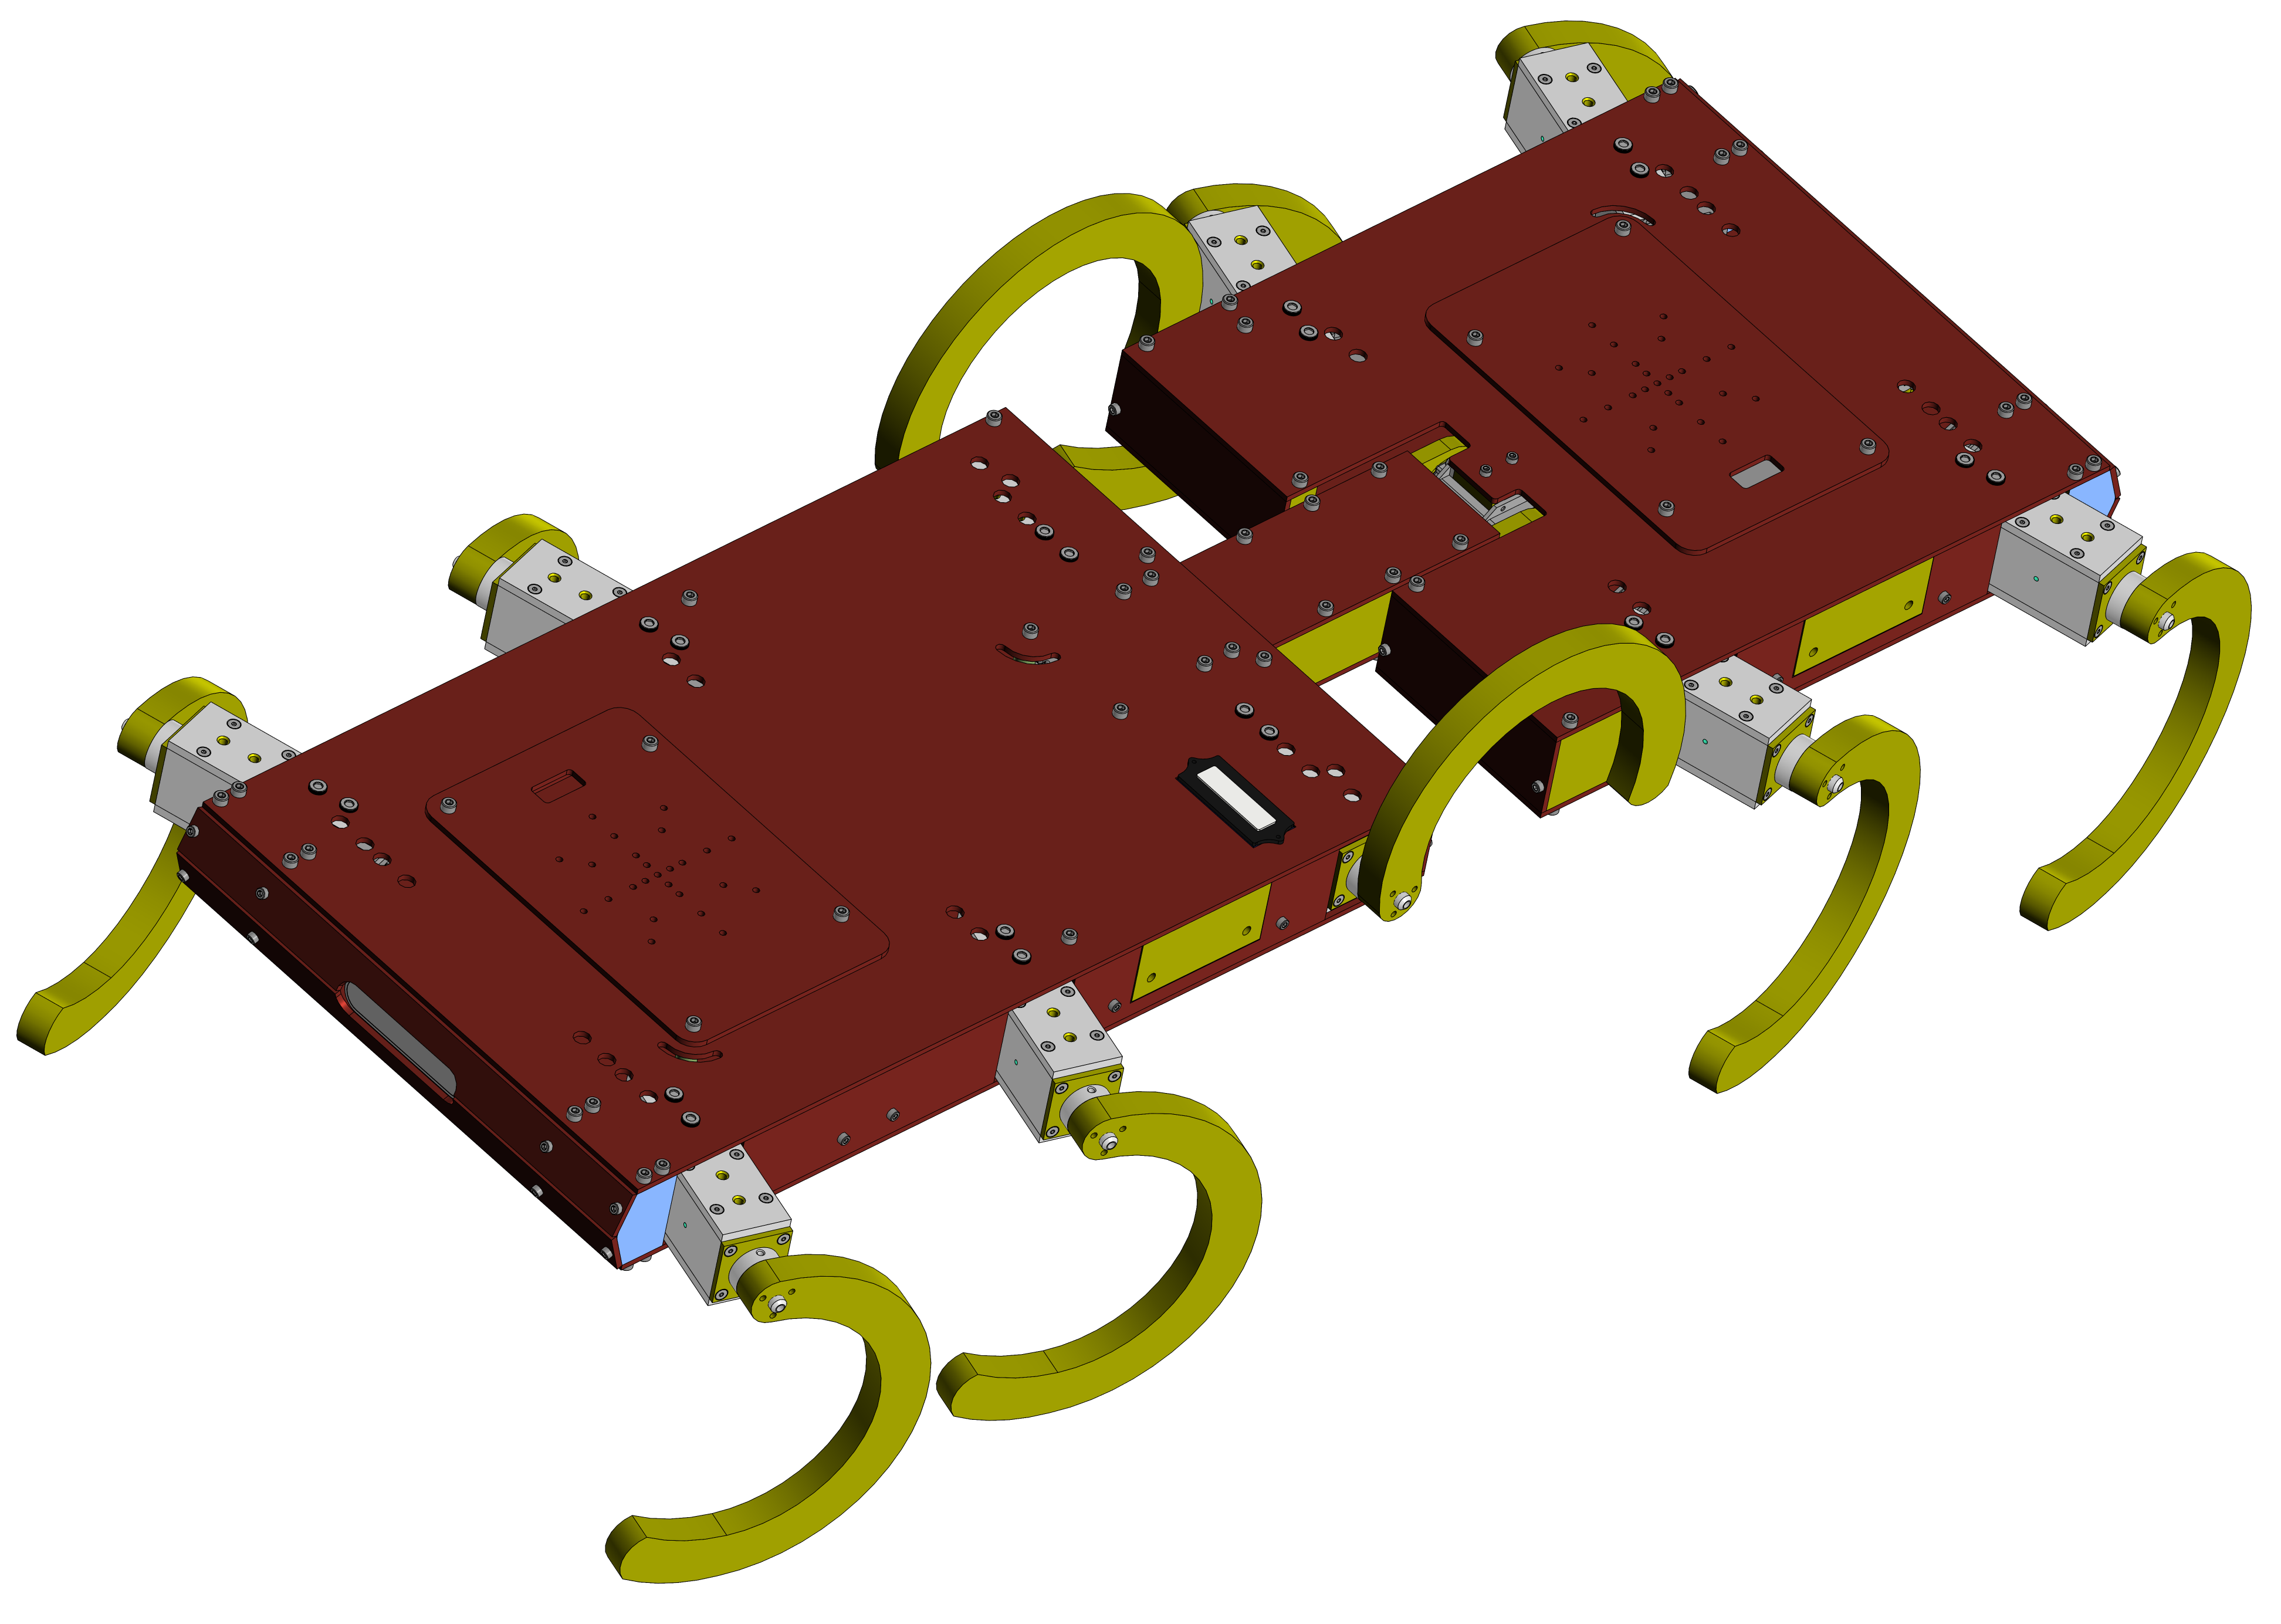
\includegraphics[height=3cm,width=1\textwidth,keepaspectratio]{strirus_4.png}
        \end{subfigure}
    \end{figure}
\end{frame}

\note{\small \setlength{\parindent}{20pt}
    
На основе полученной зависимости, разрабатывались различные прототипы. Можно выделить 5 прототипов, 2 из которых были собраны натурно. Более того, один был апробирован в приближенных к реальным условиях среде, в снегу *тык*.

Были роботы с одним и без сочленений, менялась длина ног.

Экспериментально было выяснено, что 10 но лучше, чем 12, так как при той же длине корпуса, можно сильно увеличить длину ног, что сильно влияет на профильную проходимость.
}

\begin{frame}[c]{Особенности конструкции}
    \framesubtitle{}
    \begin{figure}[H]
        \begin{subfigure}{0.39\textwidth}
            \centering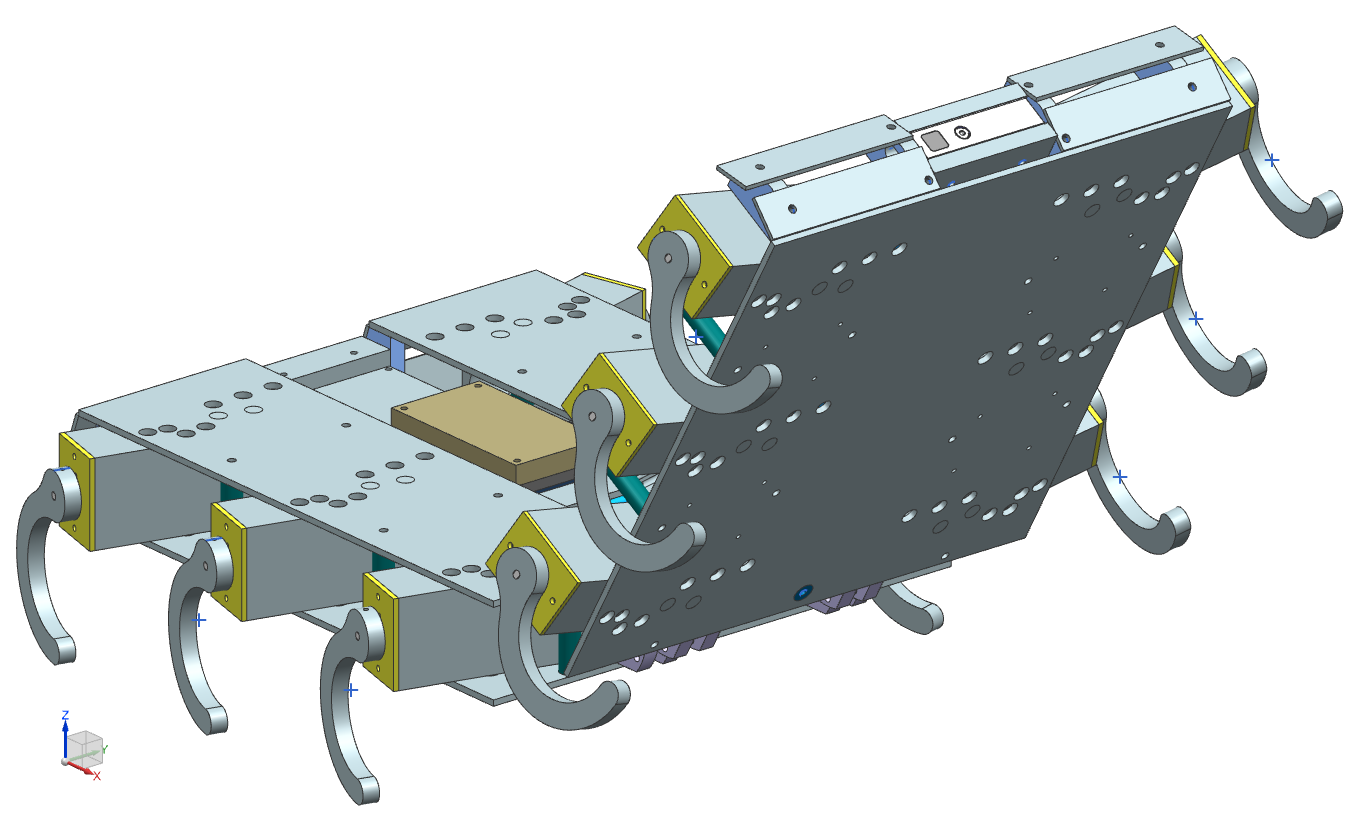
\includegraphics[height=6cm,width=1\textwidth,keepaspectratio]{17.png}
            \caption*{Одностепенной активный сегмент, соединяющий 2 части робота}
        \end{subfigure}
        \begin{subfigure}{0.59\textwidth}
            \centering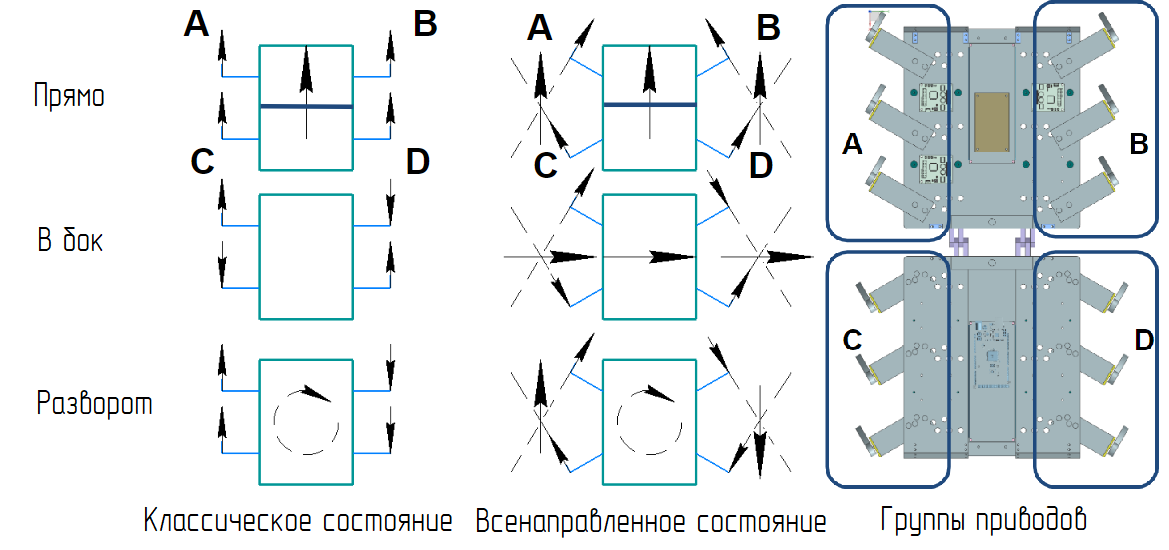
\includegraphics[height=6cm,width=1\textwidth,keepaspectratio]{vector_representation_rus}
            \caption*{Векторное представление сил в обычном и всенаправленном состояниях}
        \end{subfigure}
    \end{figure}
\end{frame}

\note{\small \setlength{\parindent}{20pt}
    
Особенности последнего прототипа в следующем. Во первых, был добавлен активный сегмент, соединяющий 2 части робота *тык*. Это позволяет добиться условия, чтобы робот мог забраться на препятствия выше себя ростом. 

Также, была придуман концепт, позволяющий двигаться такому классу роботов без смены ориентации во все стороны. Я вдохновлялся омниколесом. Справа показано как это работает. Мы разбиваем ноги робота на группы и управляя направлением вращения, можем направлять робота во все стороны *тык*. Что и показано в следующем видео.
}

\begin{frame}[t]{Четвертая итерация робота}
    \framesubtitle{}
    \begin{figure}[H]
        \centering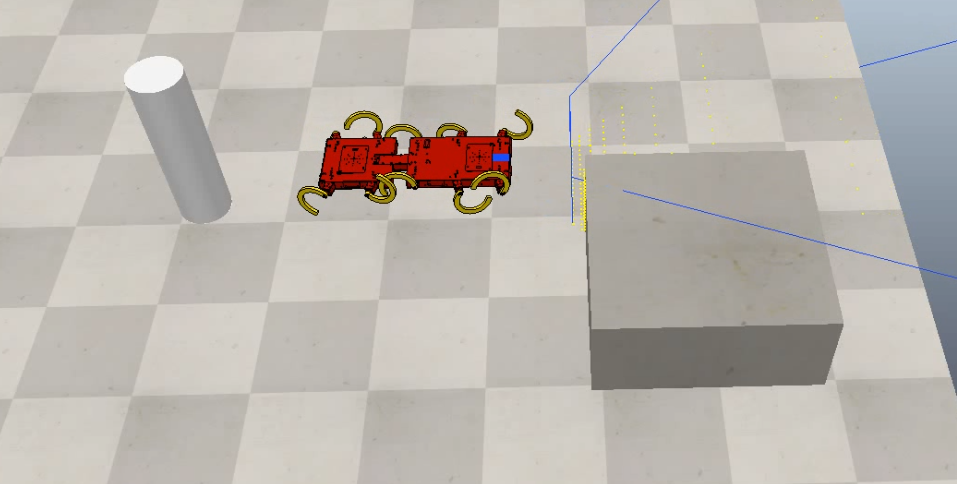
\includegraphics[height=6cm,width=1\textwidth,keepaspectratio]{sidestep_segment_video_preview.png}
    \end{figure}
\end{frame}

\note{\small \setlength{\parindent}{20pt}

На видео представлено прохождение препятствий последним прототипом робота в симуляторе CoppeliaSim}